\section{Which hidden directions the future reads}\label{sec:gramian}

Section~\ref{sec:witness} showed that some hidden angular structure returns into density, flux and stress. This section asks which, and how much, in the same linear chain, and what that means for any reduced description that keeps only the low moments.

\paragraph{The predictive quotient and its weight.} For a linear evolution $\dot v=L(\tau)v$ with readout $R$, the part of the state no readout can ever see is $N_\infty=\{v:\ RU(\tau,\tau_s)v=0\ \text{for all }\tau\}$, and the minimal summary that predicts the readout is the quotient $V/N_\infty$ (the predictive quotient of VOTKP, Theorem~3.1~\cite{VOTKP}, and of Dirac Time, Definition~1.1~\cite{DT}). Give the hidden sector an embedding $Q$ (here the moments $\ell\ge3$), the readout $R$ onto $\ell\le2$, and a horizon $T$. The readout Gramian of the hidden sector,
\begin{equation}
\mathcal G_{T}=\int_{\tau_s}^{T}Q^{\ast}U(\tau,\tau_s)^{\ast}R^{\ast}RU(\tau,\tau_s)Q\,d\tau,
\end{equation}
weighs each hidden direction $h$ by its integrated squared output, $h^\ast\mathcal G_Th$. Its kernel, as $T\to\infty$, is $N_\infty\cap\operatorname{Ran}Q$. For the neutrino chain that kernel is zero: the entry $(RB^j)_{2,2+j}=k^jc_2\cdots c_{j+1}$ of the observability matrix is nonzero for every $j$, so every hidden direction is eventually seen (Appendix~A.14). The predictive quotient of this chain is therefore the whole hidden space, and what carries information is the spectrum of $\mathcal G_T$: the directions the future reads strongly and the ones it barely reads \grade{derived}. The Gramian is the standard observability Gramian of control theory, restricted to the hidden sector; what is used here is its meaning for the predictive quotient and its use in choosing what a reduced state must keep.

\paragraph{The door, weighed.} For McCormick's history $n=3$, $\epsilon_{\rm dec}=2$ and the readout to $\epsilon=4$, profile-summed over $k$ and averaged over $\pm k$ (which makes its eigenvectors pure-parity), the top three eigenvalues are $1.1\times10^{-7}$, $9\times10^{-12}$, $10^{-15}$ for structure planted in the coupled era ($\epsilon_s=0.5$), $0.367$, $0.148$, $0.040$ at decoupling ($\epsilon_s=2$), and $0.147$, $0.024$, $0.0016$ in free streaming ($\epsilon_s=3$), the last on a shorter horizon \grade{measured; Figure~\ref{fig:gramian}}. The leading direction is always odd and led by $\ell=3$ (weight $0.92$--$0.99$, the rest mostly $\ell=5$); the second is always even and led by $\ell=4$. Halving the time step changes the leading eigenvalues by at most $3\times10^{-6}$; raising the chain to $L=90$ changes nothing at double precision. The coupled-era suppression is not the survival factor alone: it is $2.5\times10^{-9}$ against $e^{-42}$, because the damped rungs still leak through the conserved $\ell=0$ at order $(k/\sigma)^\ell$; the snapshot Gramian at the end of the horizon, which is the witness of Section~\ref{sec:witness}, follows the survival factor to within a factor of ten.

\paragraph{The direction to plant.} Among hidden perturbations that keep the intensity positive on McCormick's 32 angle bins, the one with the largest readout at the positivity edge is odd, with weights $\ell=3$: $0.851$, $\ell=5$: $0.117$, $\ell=7$: $0.010$, and gives $2.47$ times the readout of pure $p_3$ on the decoupling surface; pure $p_4$ gives $0.40$ \grade{measured}. Its shape is set by positivity; its parity and its $\ell=3$ lead are set by the Gramian. Section~\ref{sec:door} plants it in the full collapse.

\paragraph{Order, with the opacity held fixed.} Take two collision histories with the same integrated opacity $\int\sigma\,d\tau$ over a window and the rate reversed in time inside it. The optical depth is equal by construction; the time-integrated connection energy $\int\tfrac{k^2}{3}\sigma^2\,d\tau$ is equal, because it does not see order; and if the window closes before the readout, the operator at readout is equal too. The exact propagated readout is not. For six such pairs (single-rate, $n=3$ and $6$, and the split operator at $r=4$ and $1/4$), the density, flux and stress at readout differ by $33$--$72\%$, and the memory form $g_2$ by $0.06$--$0.16$, at or past the $0.08$ kill line of Section~\ref{sec:memory} \grade{measured; Figure~\ref{fig:gramian}}. The rate falling late keeps more of the kept population than the rate falling early, in every pair whose window closes before the readout. Matching optical depth between an $n=3$ and an $n=6$ history over $[0.5,4]$ still leaves $g$ differing by up to $0.74$. No scalar summary of the history, whether opacity, integrated connection energy or the operator at readout, can carry what the threshold reads; the order is part of the record. Whether the threshold itself separates such a pair is untested.

\paragraph{Closures, at linear order.} Against the exact chain, over the nine histories of Section~\ref{sec:runs}, the profile-weighted relative error of the density, flux and stress trajectories to $\epsilon=4$ falls from $P_1$ to $P_5$ in every history, and is worst for the earliest decoupling ($\epsilon_{\rm dec}=0.25$): $0.79$ for $P_1$, $0.50$ for $P_2$, $0.28$ for $P_3$, $0.071$ for $P_5$. Entropy closures add nothing at this order: linearised $M_1$ and $M_2$ are exactly $P_1$ and $P_2$. The viscous (Chapman--Enskog) closure is worst everywhere ($1.39$ at the earliest history). A short-memory correction of the optimal-prediction type~\cite{SF} beats $P_2$ in all nine. The exact elimination of the moments $\ell\ge3$ (Appendix~A.5 with the cut at $\ell=2|3$) is exact to $4.6\times10^{-6}$; freezing its kernel to one history and reusing it costs up to $0.13$ \grade{measured}. At the first compaction maximum ($\epsilon^\ast=1.7$) every truncation from $P_2$ upward gives the memory form to within $10^{-3}$; by $\epsilon^\ast=4$ they miss it by up to $0.26$. The memory is in the history of the hidden block, and an instantaneous closure on the kept moments cannot hold it.

\begin{figure}[t]\centering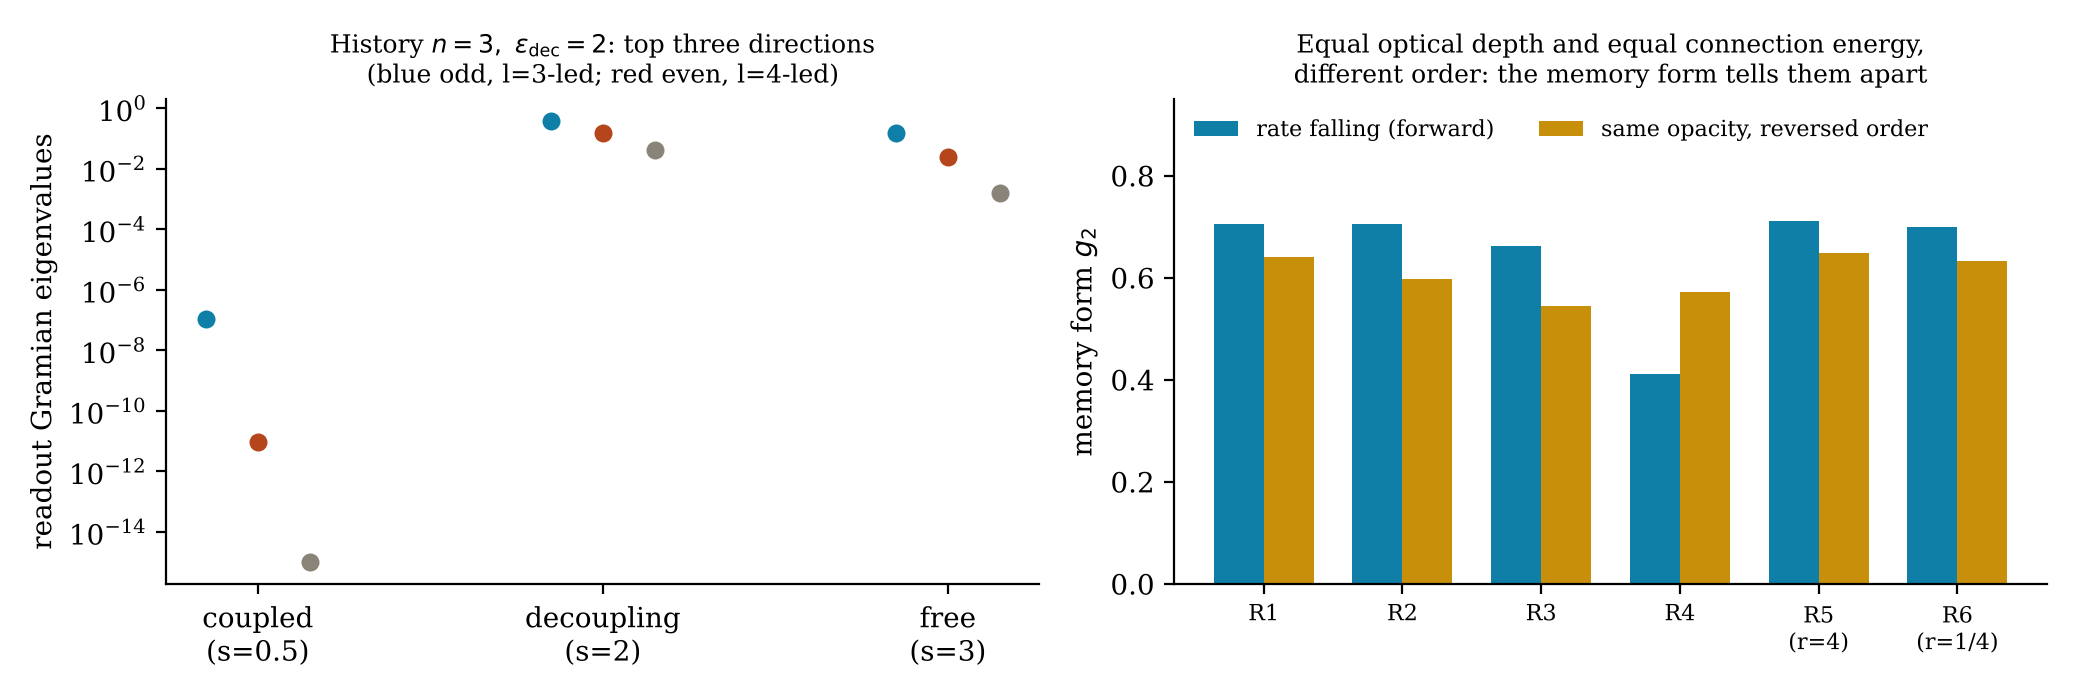
\includegraphics[width=\textwidth]{figs/fig10_gramian_order.png}
\caption{Left: eigenvalues of the readout Gramian of the hidden moments $\ell\ge3$, for structure planted in the coupled era, at decoupling and in free streaming ($n=3$, $\epsilon_{\rm dec}=2$, readout to $\epsilon=4$). Right: the memory form $g_2$ for pairs of collision histories with equal optical depth and equal integrated connection energy, the rate reversed in time inside a window; R4 is the one pair whose window contains the readout.}\label{fig:gramian}\end{figure}
